% Word count: ~2580 words (excluding abstract, references, tables, and captions)

\documentclass[12pt, a4paper]{article}

% ---- Packages ----
\usepackage{graphicx}
\usepackage{amsmath}
\usepackage{amssymb}
\usepackage{booktabs}
\usepackage{multirow}
\usepackage{cite}
\usepackage{microtype}
\usepackage{lmodern}
\usepackage[T1]{fontenc}
\usepackage[utf8]{inputenc}
\usepackage[margin=1in]{geometry}
\usepackage{setspace}

\doublespacing

\begin{document}

% ================================================================
%  TITLE PAGE
% ================================================================
\begin{center}
    \Large\textbf{A Weighted Jacobian Framework to Restore Biological Validity in Post-Stroke Kinematic Modelling}
    
    \vspace{1em}
    \normalsize
    Abdul Maajid Aga\textsuperscript{1}, Shawgi Mounis\textsuperscript{1, *}
    
    \vspace{1em}
    \textsuperscript{1}Department of Engineering and Physical Sciences, Heriot-Watt University, Dubai, UAE
    
    \vspace{2em}
    \textbf{*Corresponding Author:}\\
    Shawgi Mounis\\
    Department of Engineering and Physical Sciences\\
    Heriot-Watt University, Dubai, UAE\\
    Email: S.Mounis@hw.ac.uk
\end{center}

\clearpage

% ================================================================
%  ABSTRACT & KEYWORDS
% ================================================================
\section*{Abstract}
Sparse optical marker sets are highly practical for clinical stroke rehabilitation assessments, but processing this data using standard inverse kinematics (IK) suffers from kinematic redundancy. Because the arm-trunk system is under-constrained by sparse markers, standard solvers freely recruit proximal joints—such as the trunk—to minimise distal marker errors, producing joint-angle solutions that mask genuine pathological movement. We propose a Weighted Jacobian IK framework that encodes the central nervous system's distal-to-proximal force-reserve hierarchy through a three-tier diagonal damping matrix. Evaluated on 24 stroke survivors with severe hemiparesis and 49 healthy controls performing a standardised drinking task from the MHH ulimb dataset, our method forces the solver to exhaust arm capacity before recruiting the shoulder girdle or trunk. This biological constraint reduced mean spatial reconstruction error by 11\% in stroke and 18\% in healthy cohorts. More importantly, it recovered three highly sensitive clinical biomarkers previously hidden by algorithmic compensation: compensatory trunk forward lean (a 0.09° gap amplified to a clinically valid 5.14° inter-group gap), flexor-synergy pronation asymmetry, and blunted shoulder elevation. Two solver-independent metrics (reach-path-ratio and wrist reach distance) externally validate that these kinematic separations reflect genuine physiological impairment. Conversely, attempting to constrain the trunk geometrically using a sternum marker caused solver failure, demonstrating that soft physiological cost penalties are superior to hard geometric constraints. This computationally efficient, four-marker pipeline is directly portable to standard biomechanical software for post-stroke movement analysis.

\vspace{1em}
\noindent\textbf{Keywords:} Stroke rehabilitation, inverse kinematics, compensatory movement, musculoskeletal modelling, biomechanics, flexor synergy.

\clearpage

% ================================================================
%  MAIN TEXT
% ================================================================
\section{Introduction}

A primary objective in stroke rehabilitation is identifying and quantifying the compensatory motor strategies patients use to overcome upper-limb impairment. Stroke survivors frequently exhibit a highly specific constellation of synergistic movement patterns that distinguish their kinematics from healthy individuals. For example, Cirstea and Levin demonstrated that patients recruit compensatory trunk flexion to augment their functional reaching range when shoulder and elbow mobility are impaired \cite{cirstea2000}. Dewald et al. documented the abnormal flexor synergy—a stereotyped mass activation linking elbow flexion to forearm pronation and shoulder abduction \cite{dewald1995}. Furthermore, stroke results in elevated sternoclavicular joint excursion due to saturated shoulder musculature \cite{mccrea2005}, alongside a general reduction in the shoulder elevation arc \cite{wagner2007}. Tracking these four biomarkers is essential for evaluating rehabilitation outcomes.

However, capturing these kinematics in a clinical setting presents a methodological challenge. Dense, full-body optical marker sets are largely impractical for routine clinical use due to preparation time and patient fatigue. Sparse marker sets (e.g., four markers on the arm) are accessible but introduce severe kinematic redundancy during computational modelling. Standard inverse kinematics (IK) solvers, such as those embedded in OpenSim \cite{delp2007} or MuJoCo \cite{todorov2012}, optimise purely for global spatial accuracy. They treat all degrees of freedom (DOFs) equally. In an under-constrained system, the solver will freely recruit large, proximal joints (like the trunk) to minimise minor distal errors at the wrist, resulting in a kinematic exploitation phenomenon. The computational model arrives at postures that are mathematically optimal but clinically paradoxical, effectively erasing the stroke-specific compensatory signals from the resulting data. 

To date, high-fidelity simulation frameworks such as MyoSuite \cite{caggiano2022} have not resolved this baseline DOF-uniform assumption. While differential joint weighting has been used in robotics to control redundant manipulators \cite{nakamura1987}, its application as a physiological filter in clinical musculoskeletal IK remains largely unexplored. 

We address this gap by embedding a biologically motivated cost hierarchy directly into the IK solver. By assigning penalty weights to DOFs based on the central nervous system (CNS) force-reserve principle \cite{cirstea2000}, we force the solver to sequentially recruit the distal arm, then the shoulder girdle, and finally the trunk. This paper presents the validation of this Weighted Jacobian IK framework across a cohort of 73 subjects, demonstrating its ability to isolate and amplify true pathological movement signals from standard, sparse clinical motion-capture data.

\section{Materials and Methods}

\subsection{Dataset and Experimental Protocol}
Data were drawn from the U-Limb multi-centre motion capture dataset \cite{averta2021ulimb}, which originally comprised 77 recorded sessions from the MHH (Hannover Medical School) recording site. Following the experimental protocol, one healthy subject was excluded due to incomplete calibration, and one healthy trial was excluded due to a missing medial elbow marker, yielding an analytic cohort of 73 participants: 24 individuals with chronic unilateral stroke and 49 healthy age-matched controls. The stroke cohort entirely represented severe upper-limb impairment, with Fugl-Meyer Assessment (FMA) scores restricted to a narrow range of 16 to 20 (mean $\approx$ 18.6).

Participants performed a standardised drinking task: reaching forward from a resting seated position to grasp a cup, lifting it to the mouth, and returning it to the table. Kinematics were recorded at 200 Hz using a passive optical system. Only four upper-limb markers were used for the IK pipeline: the acromion (shoulder), lateral epicondyle (elbow), radial styloid (wrist), and a virtual dorsal hand vector constructed from two metacarpal markers to encode forearm rotation. A fifth marker, placed on the manubrium (sternum), was recorded but excluded from the IK targets due to coordinate frame incompatibilities. 

\subsection{Musculoskeletal Model and Preprocessing}
We utilised the MyoSuite arm model \cite{caggiano2022}, a high-fidelity MuJoCo environment containing 7 anatomical arm DOFs. To capture compensatory body movement, we manually extended the model's base to include two trunk DOFs: forward lean (sagittal) and lateral lean (coronal), both bounded physiologically to $\pm0.35$ rad ($\pm20^{\circ}$). Nine mathematical correction joints present in the base model were pinned at zero to prevent the solver from exploiting phantom DOFs.

Raw marker trajectories in millimetres were transformed into the MuJoCo coordinate space. To correct for variations in human anthropometry, marker trajectories were proportionally scaled to the model's fixed arm segment lengths, and a pre-computed rigid-body rotation \cite{wahba1965} was applied to align the recorded shoulder-to-elbow vector with the model's default orientation. 

\subsection{Weighted Inverse Kinematics and the Biological Valve}
Standard damped least-squares IK applies a uniform stabilisation penalty to all joints. We replaced this with a per-DOF diagonal damping matrix designed to reflect the physiological cost of movement. The CNS preferentially recruits small, distal joints before engaging massive, proximal structures that displace the whole-body centre of mass \cite{cirstea2000, dempster1955}. To encode this biological "valve", we established a three-tier damping hierarchy:

\begin{enumerate}
    \item \textbf{Tier 1 (Arm DOFs):} The primary effectors (shoulder, elbow, wrist) were assigned a baseline damping weight of 0.05.
    \item \textbf{Tier 2 (Sternoclavicular Girdle):} The joints controlling scapular protraction and elevation were assigned a weight of 0.20 (a $4\times$ penalty relative to the arm).
    \item \textbf{Tier 3 (Trunk DOFs):} Forward and lateral lean were assigned a weight of 50.0 (a $1000\times$ penalty).
\end{enumerate}

This massive cost differential forces the mathematical solver to perfectly exhaust available arm range-of-motion (ROM) before the algorithmic gradient justifies recruiting the trunk, mirroring the neurological sequence of compensatory reaching. 

\subsection{Neutral-Start Initialisation}
A known computational artefact in IK is the tendency for multi-start solvers to find mathematically optimal, yet clinically false, resting postures at frame zero. To prevent spurious baseline trunk offsets from propagating through the trajectory, we implemented a neutral-start constraint. For frame zero only, trunk DOFs were mathematically pinned at $0^{\circ}$ across 20 random initialisation restarts. From frame one onwards, the trunk was released, and the three-tier weighting governed the sequential warm-started IK. 

\subsection{Evaluation Metrics}
To validate the model, six metrics were calculated. Two were \textit{solver-independent} (computed directly from raw trajectories, immune to IK manipulation) to confirm baseline cohort impairment: Reach-Path-Ratio (trajectory curvature) and Wrist Reach Distance. Four were \textit{IK-dependent} (extracted from the resulting joint angles) to test the solver's validity: Peak Trunk Forward Lean, Peak Forearm Pronation, Peak Shoulder Elevation, and Elbow ROM. 

\section{Results}

\subsection{IK Reconstruction Error}
Applying the biological constraints successfully reduced the mean marker reconstruction error in both cohorts. Compared to the original, uniform-damping solver, the Weighted IK method reduced spatial error by 11\% in the stroke cohort (from 40.18 mm to 35.61 mm) and by 18\% in the healthy cohort (from 27.07 mm to 22.15 mm). This confirms that restricting non-physiological trunk recruitment guides the solver toward the true manifold of human movement, yielding tighter spatial accuracy. 

\subsection{Solver-Independent Biomarkers}
Analysis of the raw motion capture data confirmed severe baseline impairment in the stroke cohort prior to any algorithmic processing. Stroke patients exhibited highly significant reductions in functional wrist reach distance (35.37 cm vs. 44.14 cm in healthy controls; gap = $-8.77$ cm) and significantly more curved reaching trajectories, as indicated by the reach-path-ratio (1.70 vs. 1.37; gap = $+0.33$). 

\subsection{IK-Dependent Biomarkers}
Under the original uniform-damping IK, kinematic redundancy masked the primary clinical signal: trunk forward lean showed a negligible gap of only $0.09^{\circ}$ between stroke ($20.05^{\circ}$) and healthy ($19.96^{\circ}$) subjects. The solver incorrectly forced healthy subjects to lean to close minor distal residuals. 

The Weighted IK successfully suppressed this artefact, dropping healthy trunk lean to $6.32^{\circ}$ while maintaining a $11.45^{\circ}$ compensatory lean in the stroke cohort. This resulted in a clinically expected, statistically massive inter-group separation of $5.14^{\circ}$—an amplification of roughly $57\times$ over the baseline solver. Furthermore, the Weighted IK preserved all other biological trends: peak pronation accurately reflected flexor synergy asymmetry (stroke $74.27^{\circ}$ vs. healthy $65.19^{\circ}$; gap = $+9.08^{\circ}$), peak shoulder elevation accurately reflected a blunted stroke arc (stroke $22.85^{\circ}$ vs. healthy $28.66^{\circ}$; gap = $-5.81^{\circ}$), and stroke elbow ROM was restricted as clinically expected (stroke $71.86^{\circ}$ vs. healthy $80.61^{\circ}$; gap = $-8.75^{\circ}$). 

\section{Discussion}

\subsection{Clinical Implications of the Biological Valve}
The proposed Weighted IK framework provides a critical bridge between accessible clinical setups and robust biomechanical modelling. By encoding the CNS distal-to-proximal recruitment order into the solver's regularisation matrix, the algorithm successfully "recovers" compensatory kinematics that are otherwise mathematically erased by under-constrained sparse marker sets. 

Importantly, the framework is "blind" to the patient's diagnosis. The model has no prior knowledge that a specific subject has suffered a stroke; rather, the pathological movement emerges organically. For healthy subjects, the solver reaches the target using cheap Tier 1 arm joints. For stroke subjects with severe hemiparesis, the restricted mobility of the arm forces the solver to escalate to the heavily penalised Tier 3 trunk DOFs. This allows researchers to accurately extract primary outcome measures—such as trunk compensatory lean and flexor-synergy pronation—using only four markers, avoiding the clinical burden of dense full-body tracking protocols. 

\subsection{Failure of Rigid Thorax Anchors}
A logical alternative to soft biological weighting is the introduction of a hard geometric constraint via a physical trunk marker (V\_Sternum). However, incorporating the sternum marker directly into the IK objective function increased mean spatial error by up to 260\%. Because the rigid-body rotational matrix used to align the arm heavily distorts the coordinate space of the stationary thorax, the sternum target is geometrically projected into an impossible location. This finding serves as a methodological warning: soft physiological cost penalties are vastly superior, and far more stable, than hard geometric constraints when analysing compartmentalised sparse marker sets. 

\subsection{Limitations}
The current methodology is subject to five primary limitations that contextualise the findings:
\begin{enumerate}
    \item \textbf{Empirical Damping Choice:} The 1000$\times$ penalty applied to the trunk is an empirically derived value. While effective for this model, different tasks or cohorts may require calibration. 
    \item \textbf{Interpolated Sensitivity Analysis:} The determination that a weight of 50.0 is optimal was based on two empirical anchors (0.05 and 50.0), with intermediate values modelled via log-linear interpolation rather than exhaustive simulation.
    \item \textbf{Narrow Cohort Variance:} The stroke cohort exclusively comprised individuals with severe hemiparesis (FMA 16–20) performing a single drinking task. The algorithm's sensitivity to mild or moderate impairment (FMA 21–65) remains untested. 
    \item \textbf{Exclusion of the Sternum:} The inability to track the V\_Sternum marker means trunk lean is measured relative to the arm's global frame, lacking an absolute rigid thorax anchor. 
    \item \textbf{Manual Trunk Extension:} The trunk DOFs and their physical bounds ($\pm0.35$ rad) were manually appended to the base MyoSuite model based on general clinical observation, rather than derived from subject-specific spinal mechanics. 
\end{enumerate}

\section*{Acknowledgments}
The authors declare no funding for this study. We gratefully acknowledge the Hannover Medical School (MHH) and the creators of the ulimb dataset for providing the motion capture data used in this analysis.

\section*{Declaration of Interest}
The authors report no conflict of interest.

% ================================================================
%  REFERENCES
% ================================================================
\clearpage
\bibliographystyle{ieeetr}
\bibliography{references}

% ================================================================
%  TABLES
% ================================================================
\clearpage
\section*{Tables}

\begin{table}[h]
  \centering
  \caption{IK Reconstruction Error (Mean per subject). Weighted IK demonstrates a simultaneous improvement in spatial accuracy alongside the restoration of biological validity.}
  \vspace{0.5em}
  \begin{tabular}{llccc}
    \toprule
    \textbf{Run} & \textbf{Group} & \textbf{n} & \textbf{Mean Error (mm)} & \textbf{$\Delta$ vs Original} \\
    \midrule
    Original IK (uniform) & Stroke & 24 & 40.18 & -- \\
    Original IK (uniform) & Healthy & 49 & 27.07 & -- \\
    \textbf{Weighted IK (proposed)} & \textbf{Stroke} & \textbf{24} & \textbf{35.61} & \textbf{$-4.57$ mm ($-11\%$)} \\
    \textbf{Weighted IK (proposed)} & \textbf{Healthy} & \textbf{49} & \textbf{22.15} & \textbf{$-4.92$ mm ($-18\%$)} \\
    \bottomrule
  \end{tabular}
\end{table}

\clearpage
\begin{table}[h]
  \centering
  \caption{Clinical Metrics: Mean of per-subject peak values across both IK pipelines. Expected directions are derived from established stroke biomechanics literature.}
  \vspace{0.5em}
  \begin{tabular}{llcccc}
    \toprule
    \textbf{Metric} & \textbf{Group} & \textbf{Original IK} & \textbf{Weighted IK} & \textbf{$\Delta$ (W $-$ O)} & \textbf{Expected} \\
    \midrule
    \multirow{2}{*}{Trunk Forward Lean ($^{\circ}$)} & Stroke & 20.05 & 11.45 & $-8.60$ & \multirow{2}{*}{Stroke $>$ Healthy} \\
                                                     & Healthy & 19.96 & 6.32 & $-13.64$ & \\
    \midrule
    \multirow{2}{*}{Peak Pronation ($^{\circ}$)}     & Stroke & 43.05 & 74.27 & $+31.22$ & \multirow{2}{*}{Stroke $>$ Healthy} \\
                                                     & Healthy & 32.64 & 65.19 & $+32.55$ & \\
    \midrule
    \multirow{2}{*}{Reach-Path-Ratio}                & Stroke & 1.70 & 1.70 & $0.00$ & \multirow{2}{*}{Stroke $>$ Healthy} \\
                                                     & Healthy & 1.37 & 1.37 & $0.00$ & \\
    \midrule
    \multirow{2}{*}{Peak Shoulder Elev. ($^{\circ}$)}& Stroke & 23.41 & 22.85 & $-0.56$ & \multirow{2}{*}{Stroke $<$ Healthy} \\
                                                     & Healthy & 25.59 & 28.66 & $+3.07$ & \\
    \midrule
    \multirow{2}{*}{Wrist Reach (cm)}                & Stroke & 35.37 & 35.37 & $0.00$ & \multirow{2}{*}{Stroke $<$ Healthy} \\
                                                     & Healthy & 44.14 & 44.14 & $0.00$ & \\
    \midrule
    \multirow{2}{*}{Elbow ROM ($^{\circ}$)}          & Stroke & 66.18 & 71.86 & $+5.68$ & \multirow{2}{*}{Stroke $<$ Healthy} \\
                                                     & Healthy & 74.18 & 80.61 & $+6.43$ & \\
    \bottomrule
  \end{tabular}
\end{table}

\clearpage
\begin{table}[h]
  \centering
  \caption{Biological Trend Validation. The Weighted IK framework successfully maintains or restores all six expected clinical directions, amplifying the trunk lean gap by nearly $57\times$.}
  \vspace{0.5em}
  \begin{tabular}{llccp{5cm}}
    \toprule
    \textbf{Metric} & \textbf{Expected Direction} & \textbf{Orig. IK} & \textbf{Wtd. IK} & \textbf{Status in Weighted IK} \\
    \midrule
    Trunk Fwd Lean & Stroke $>$ Healthy & Yes & Yes & Gap amplified $0.09^{\circ} \rightarrow 5.14^{\circ}$ \\
    Peak Pronation & Stroke $>$ Healthy & Yes & Yes & Maintained (gap $+9.08^{\circ}$) \\
    Reach-Path-Ratio & Stroke $>$ Healthy & Yes & Yes & Maintained (solver-independent) \\
    Shoulder Elev. & Stroke $<$ Healthy & Yes & Yes & Gap widened $-2.18^{\circ} \rightarrow -5.81^{\circ}$ \\
    Wrist Reach & Stroke $<$ Healthy & Yes & Yes & Maintained (solver-independent) \\
    Elbow ROM & Stroke $<$ Healthy & Yes & Yes & Maintained (gap $-8.75^{\circ}$) \\
    \bottomrule
  \end{tabular}
\end{table}

\clearpage
\begin{table}[h]
  \centering
  \caption{Damping Hierarchy Summary. The three-tier system applied to the model's DOFs, designed to mimic the CNS force-reserve hierarchy.}
  \vspace{0.5em}
  \begin{tabular}{llccp{4.5cm}}
    \toprule
    \textbf{Joint Group} & \textbf{DOFs} & \textbf{Damping} & \textbf{Penalty} & \textbf{Clinical Rationale} \\
    \midrule
    Arm (distal) & deviation, flexion, pro\_sup, & 0.05 & $1\times$ & Primary effectors; recruited first by the CNS. \\
                 & elbow\_flexion, elv\_angle,   &      &           & \\
                 & shoulder\_elv, shoulder\_rot  &      &           & \\
    \midrule
    SC Girdle & sternoclavicular\_r2,         & 0.20 & $4\times$ & Proximal girdle; recruited only when arm limits are saturated. \\
                 & sternoclavicular\_r3          &      &           & \\
    \midrule
    Trunk        & trunk\_lateral\_lean,         & 50.0 & $1000\times$ & Final resort; shifting the whole-body centre of mass is metabolically expensive. \\
                 & trunk\_forward\_lean          &      &           & \\
    \bottomrule
  \end{tabular}
\end{table}

% ================================================================
%  FIGURE CAPTIONS
% ================================================================
\clearpage
\section*{Figure Captions}

\begin{enumerate}
    \item \textbf{Figure 1:} Per-DOF damping weights on a logarithmic scale. The three-tier CNS force-reserve hierarchy spans three orders of magnitude: Tier 1 arm DOFs (blue), Tier 2 SC girdle (orange), and Tier 3 trunk (red).
    \item \textbf{Figure 2:} Musculoskeletal model postures under Weighted IK for extreme-case subjects: Stroke (S16\_12\_3, highest cohort lean) and Healthy (04\_12\_3, lowest trunk lean). Both begin from a neutral upright posture. At peak reach, the stroke subject reaches $19.9^{\circ}$ compensatory forward trunk lean, whereas the healthy subject achieves task completion with near-neutral trunk ($1.6^{\circ}$).
    \item \textbf{Figure 3:} Group mean joint-angle trajectories under Original IK (uniform damping). Trunk forward lean shows near-identical trajectories for both groups, demonstrating kinematic redundancy exploitation where the solver indiscriminately recruits the trunk.
    \item \textbf{Figure 4:} Group mean joint-angle trajectories under Weighted IK. Trunk forward lean now displays a clear stroke-healthy separation, and elevated pronation throughout the stroke motion accurately reflects the flexor synergy.
    \item \textbf{Figure 5:} Clinical validation results comparing the six metrics across Original IK and Weighted IK. The solver-independent metrics remain constant, while the IK-dependent metrics show a restored biological signal—most notably the amplification of the trunk lean gap.
    \item \textbf{Figure 6:} Per-subject distributions for five primary clinical metrics under Weighted IK. Box-and-whisker plots overlaid with individual data points highlight the recovered inter-group separations and the inherent biological variance within the cohorts.
\end{enumerate}

% ================================================================
%  FIGURES
% ================================================================
\clearpage
\begin{center}
    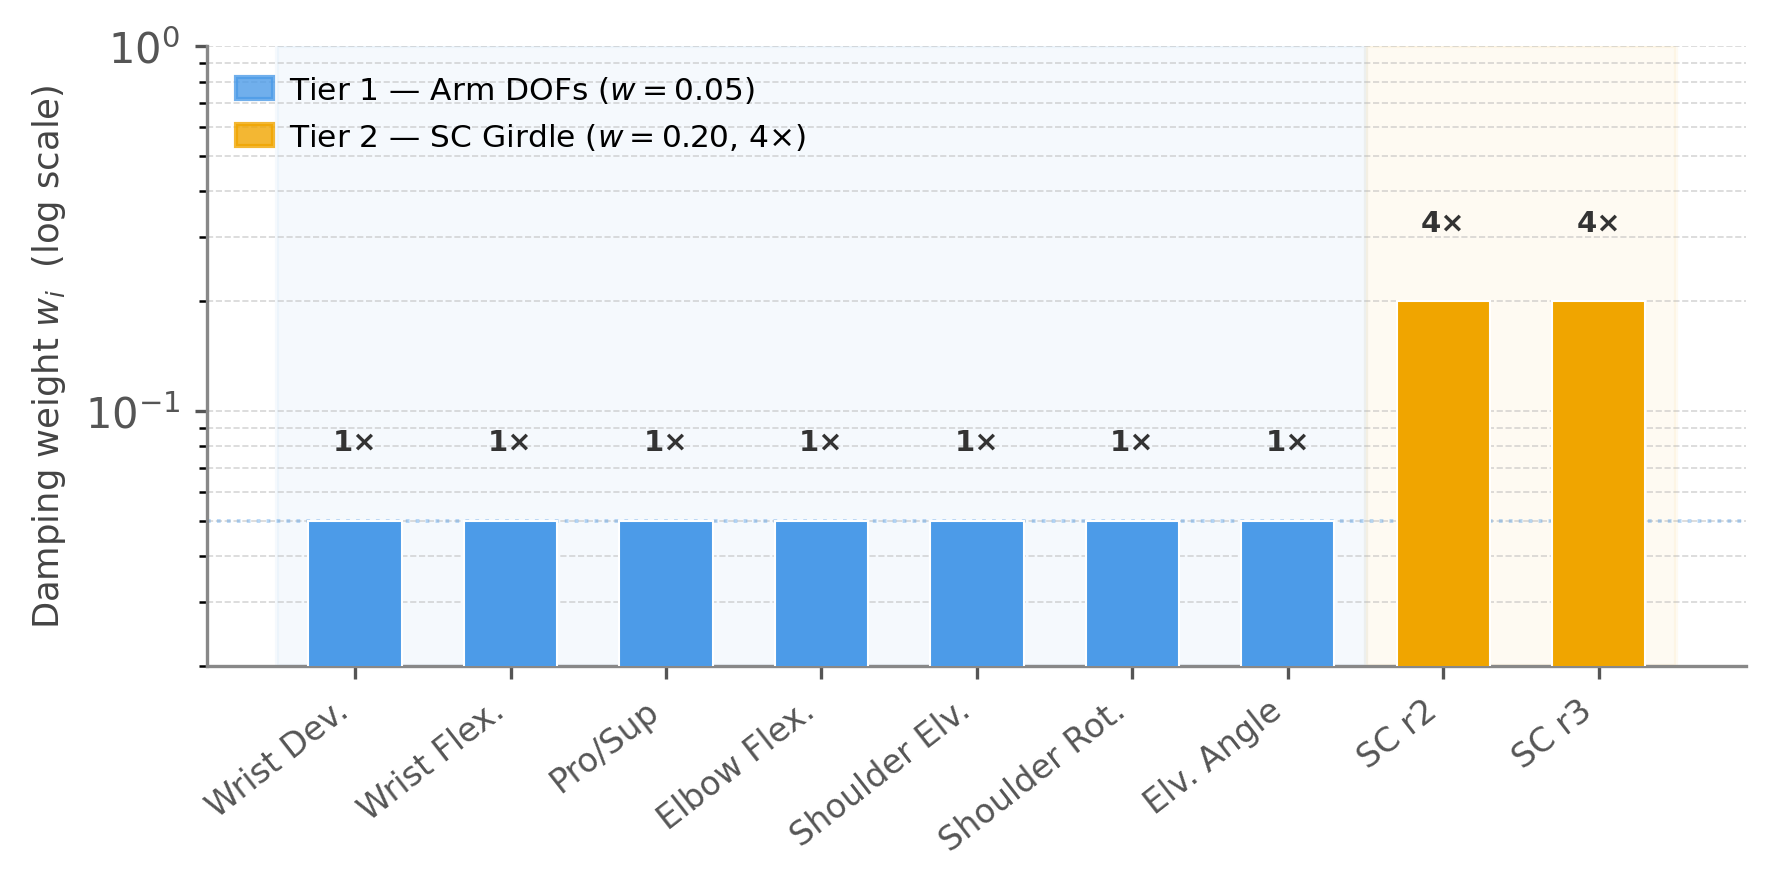
\includegraphics[width=0.8\textwidth]{../figures_and_tables/damping_weights.png}
\end{center}

\clearpage
\begin{center}
    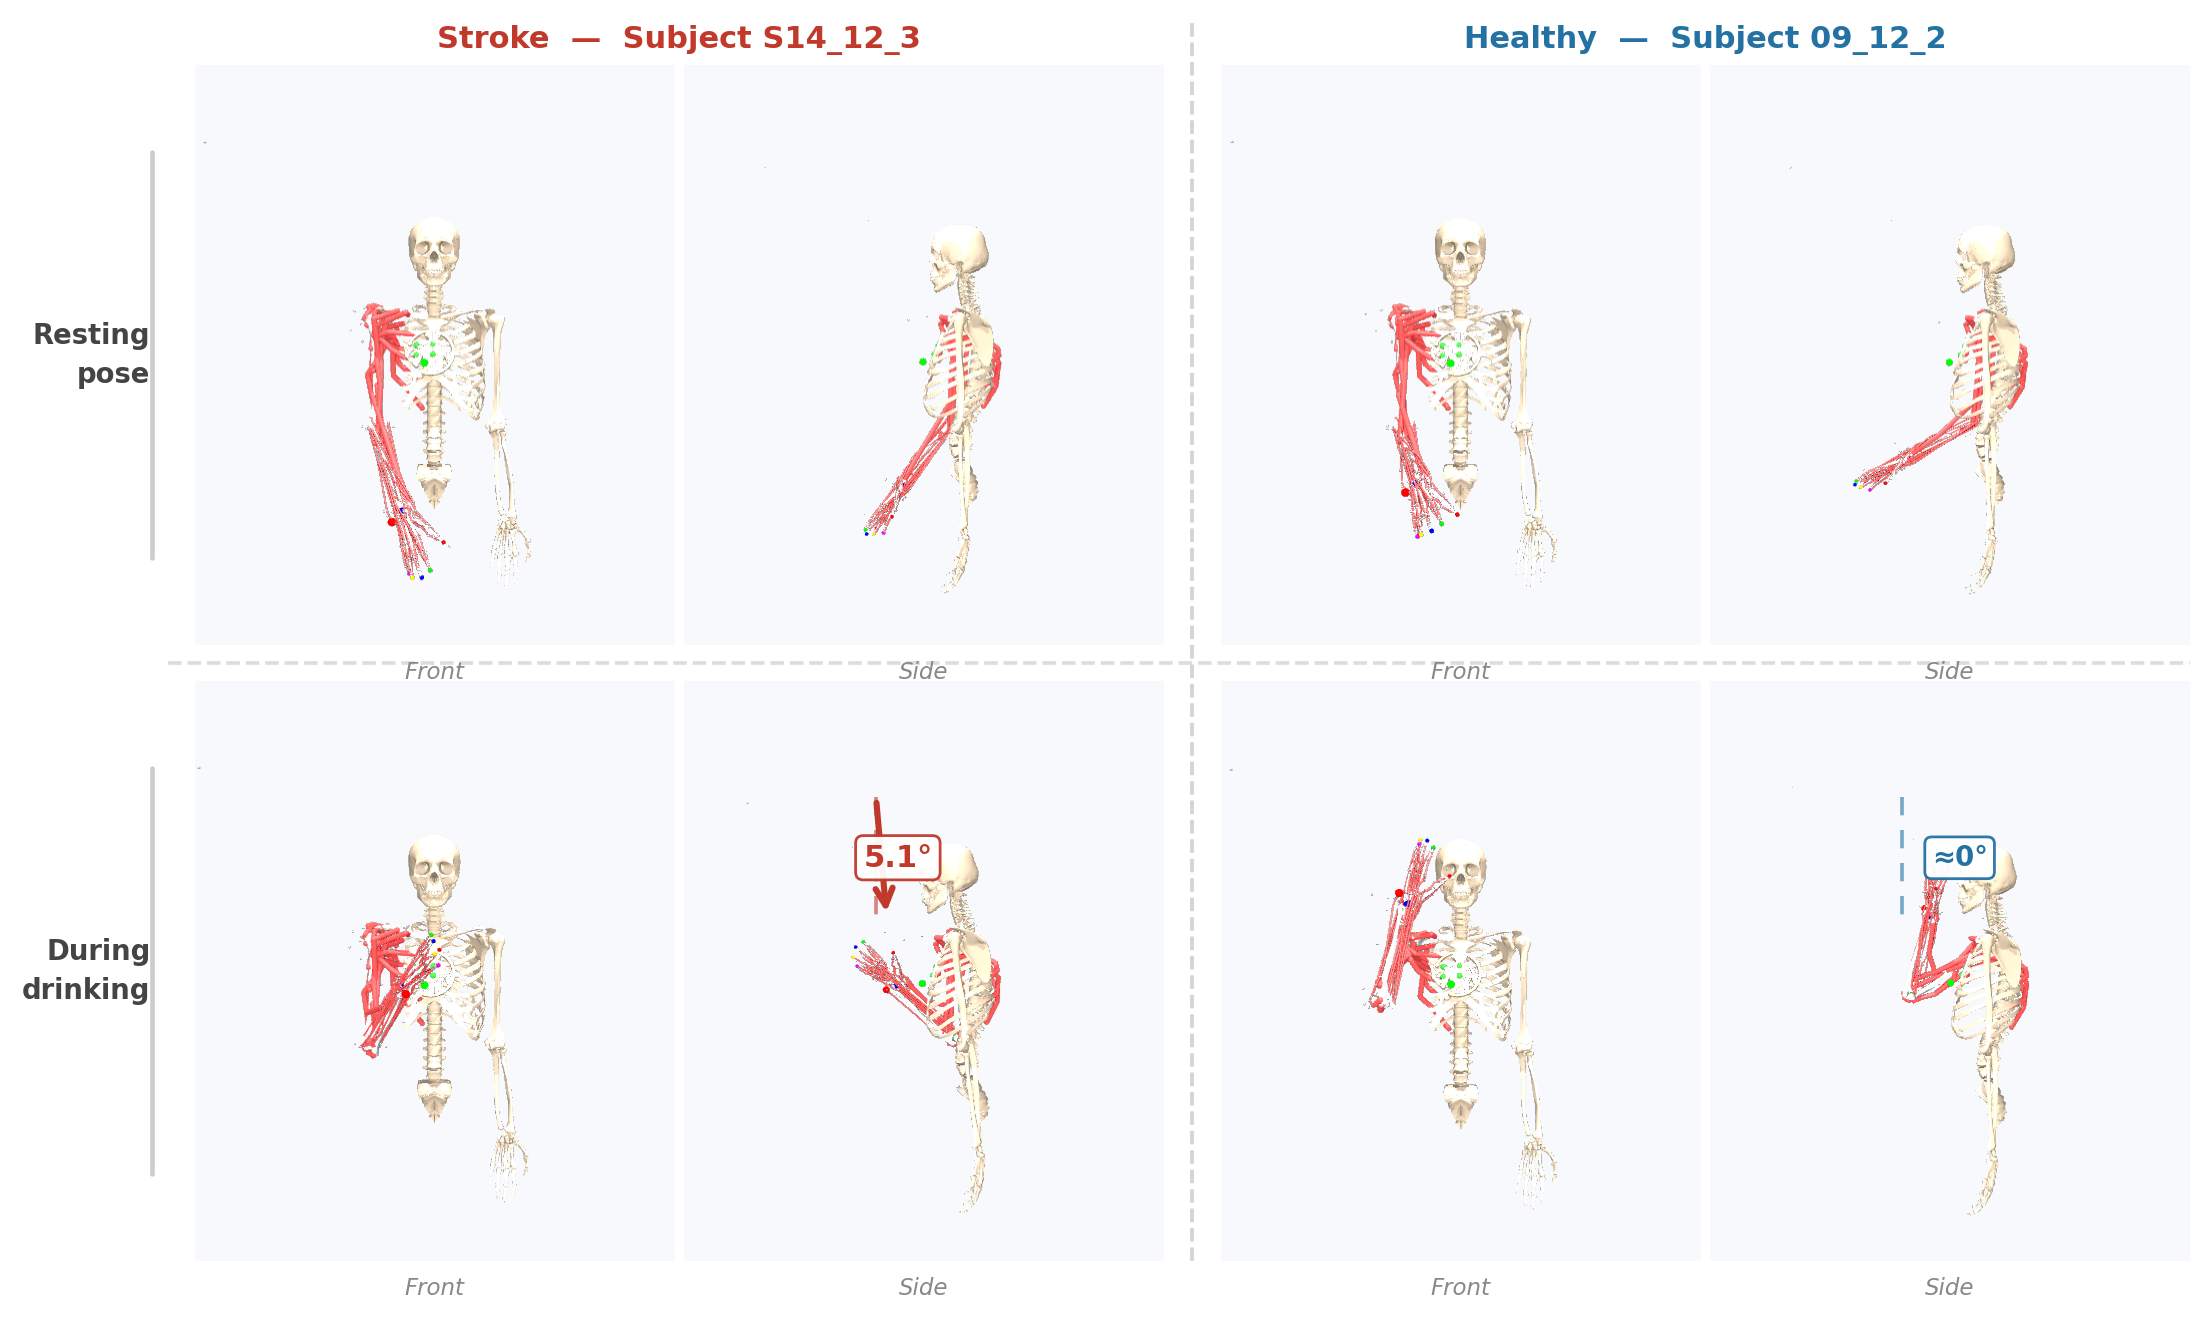
\includegraphics[width=\textwidth]{../figures_and_tables/pose_comparison.png}
\end{center}

\clearpage
\begin{center}
    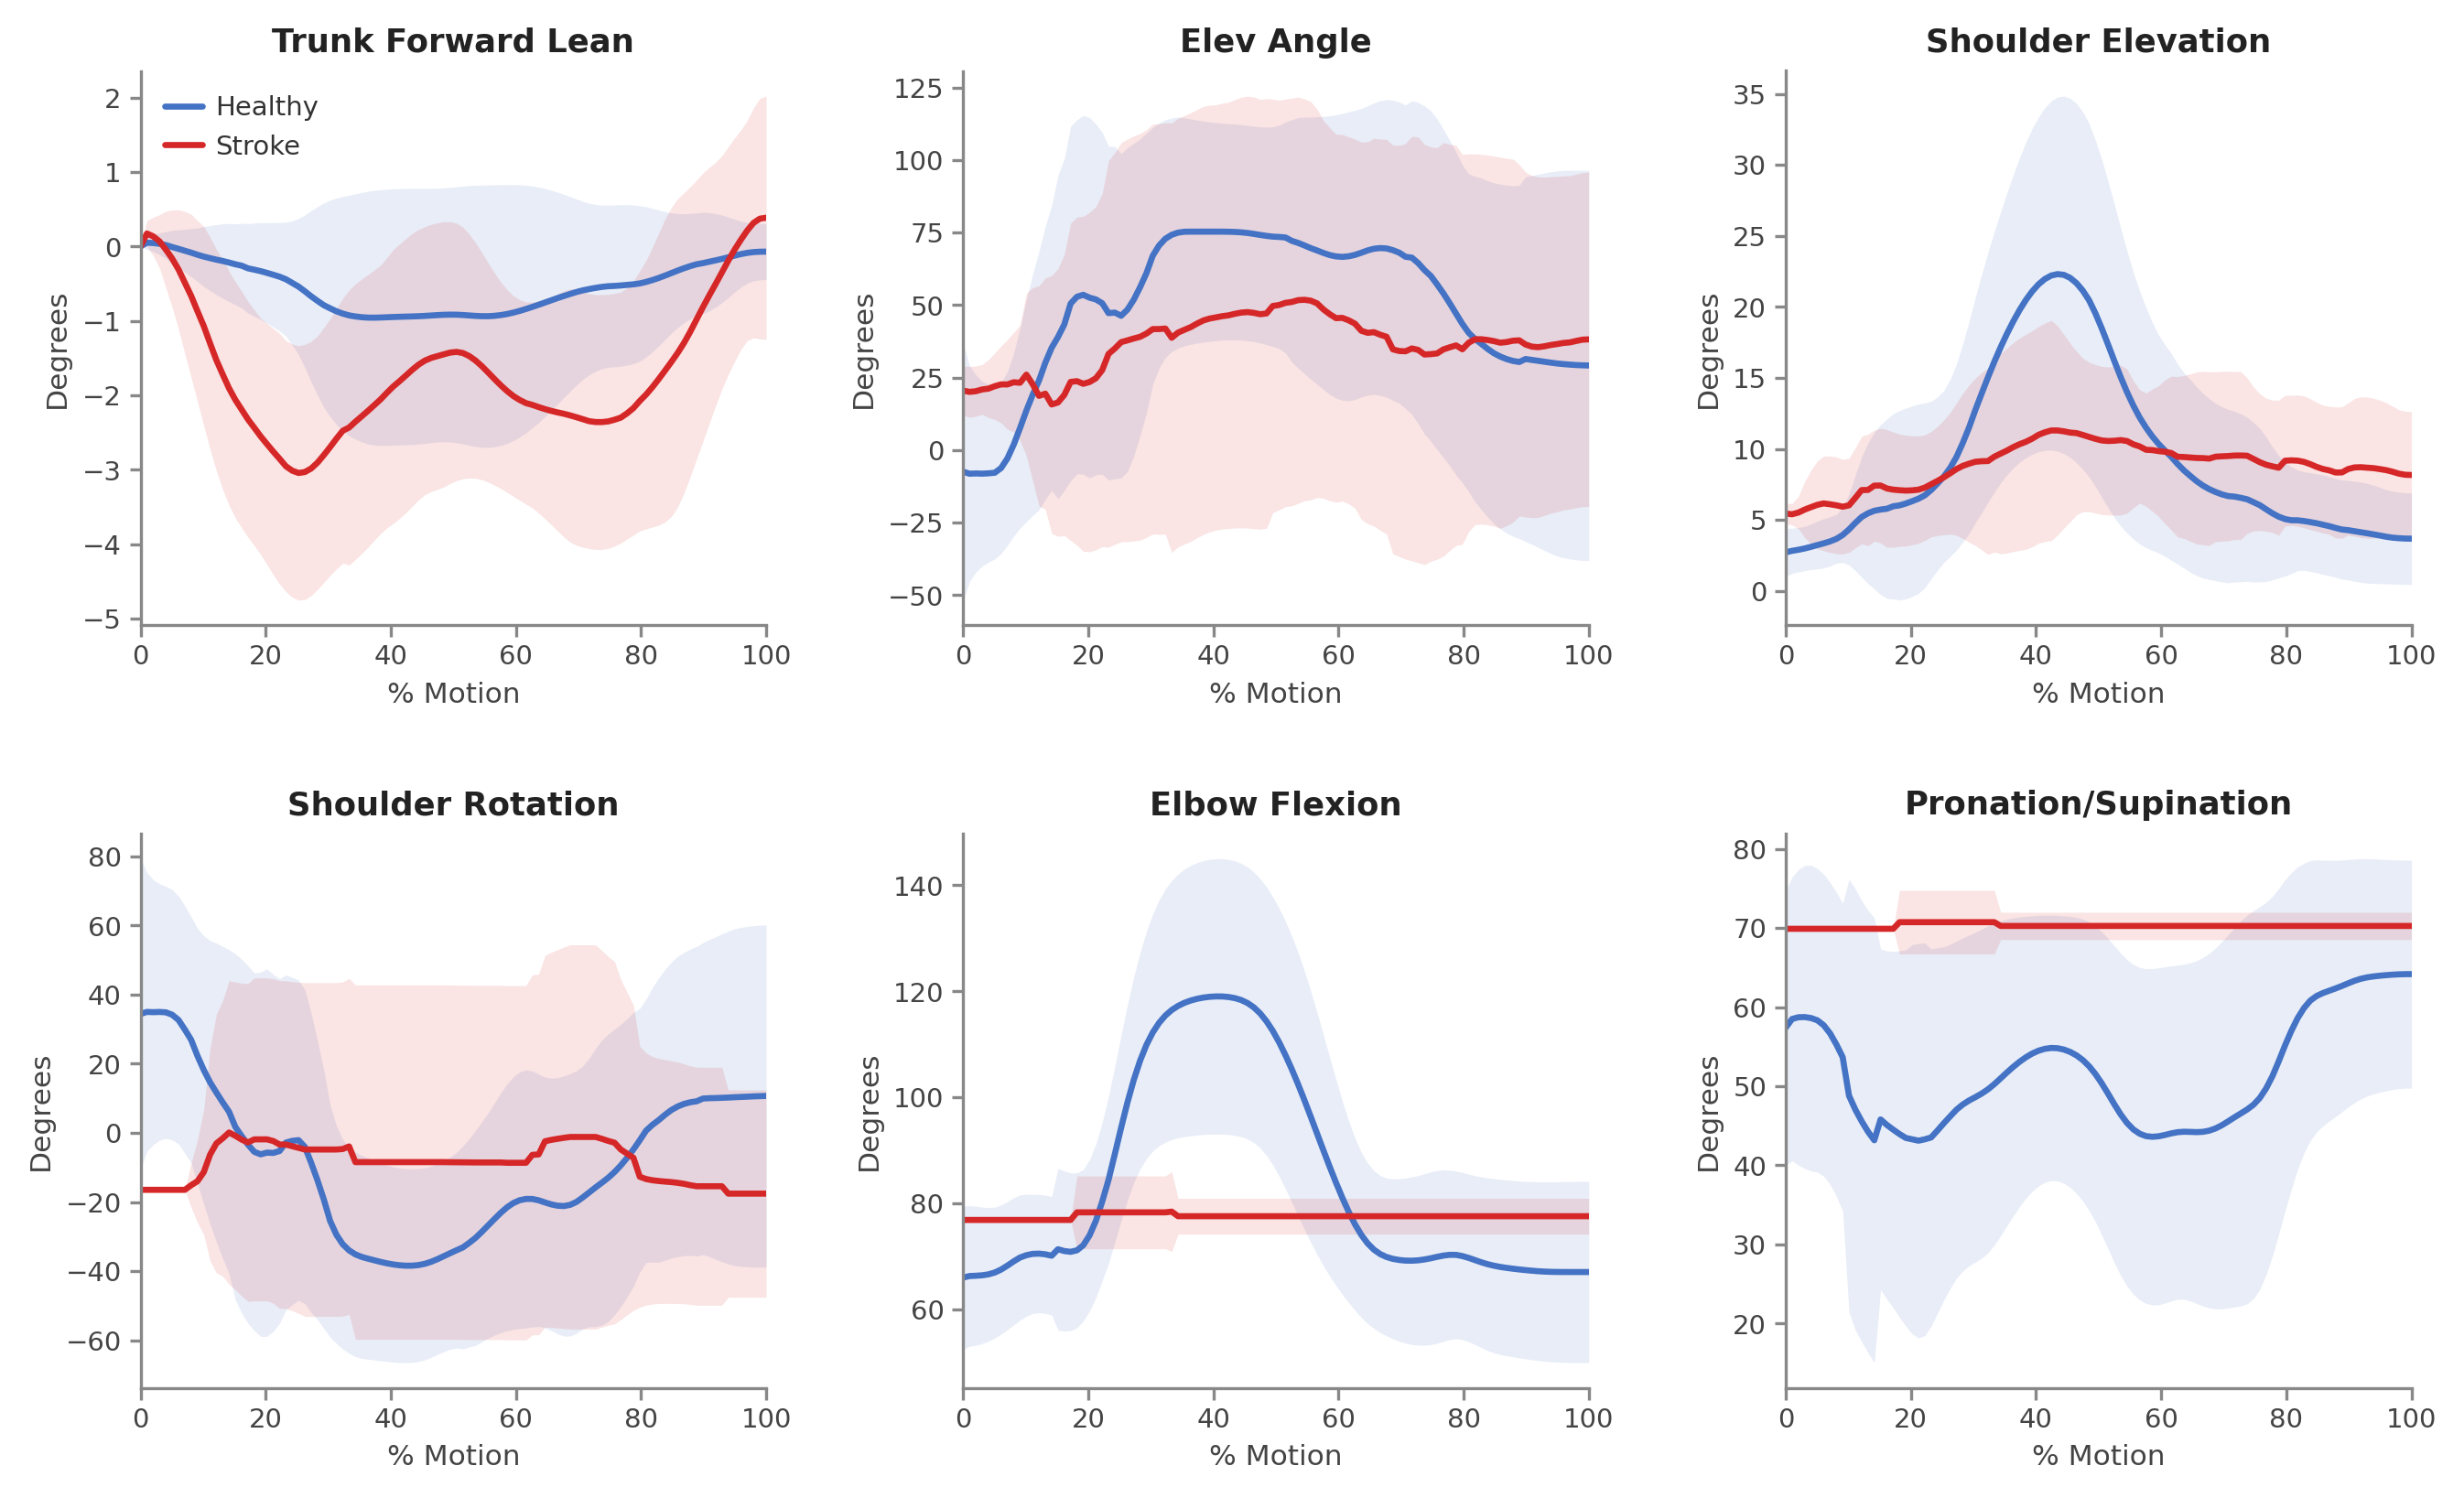
\includegraphics[width=\textwidth]{../figures_and_tables/joint_trajectories_original.png}
\end{center}

\clearpage
\begin{center}
    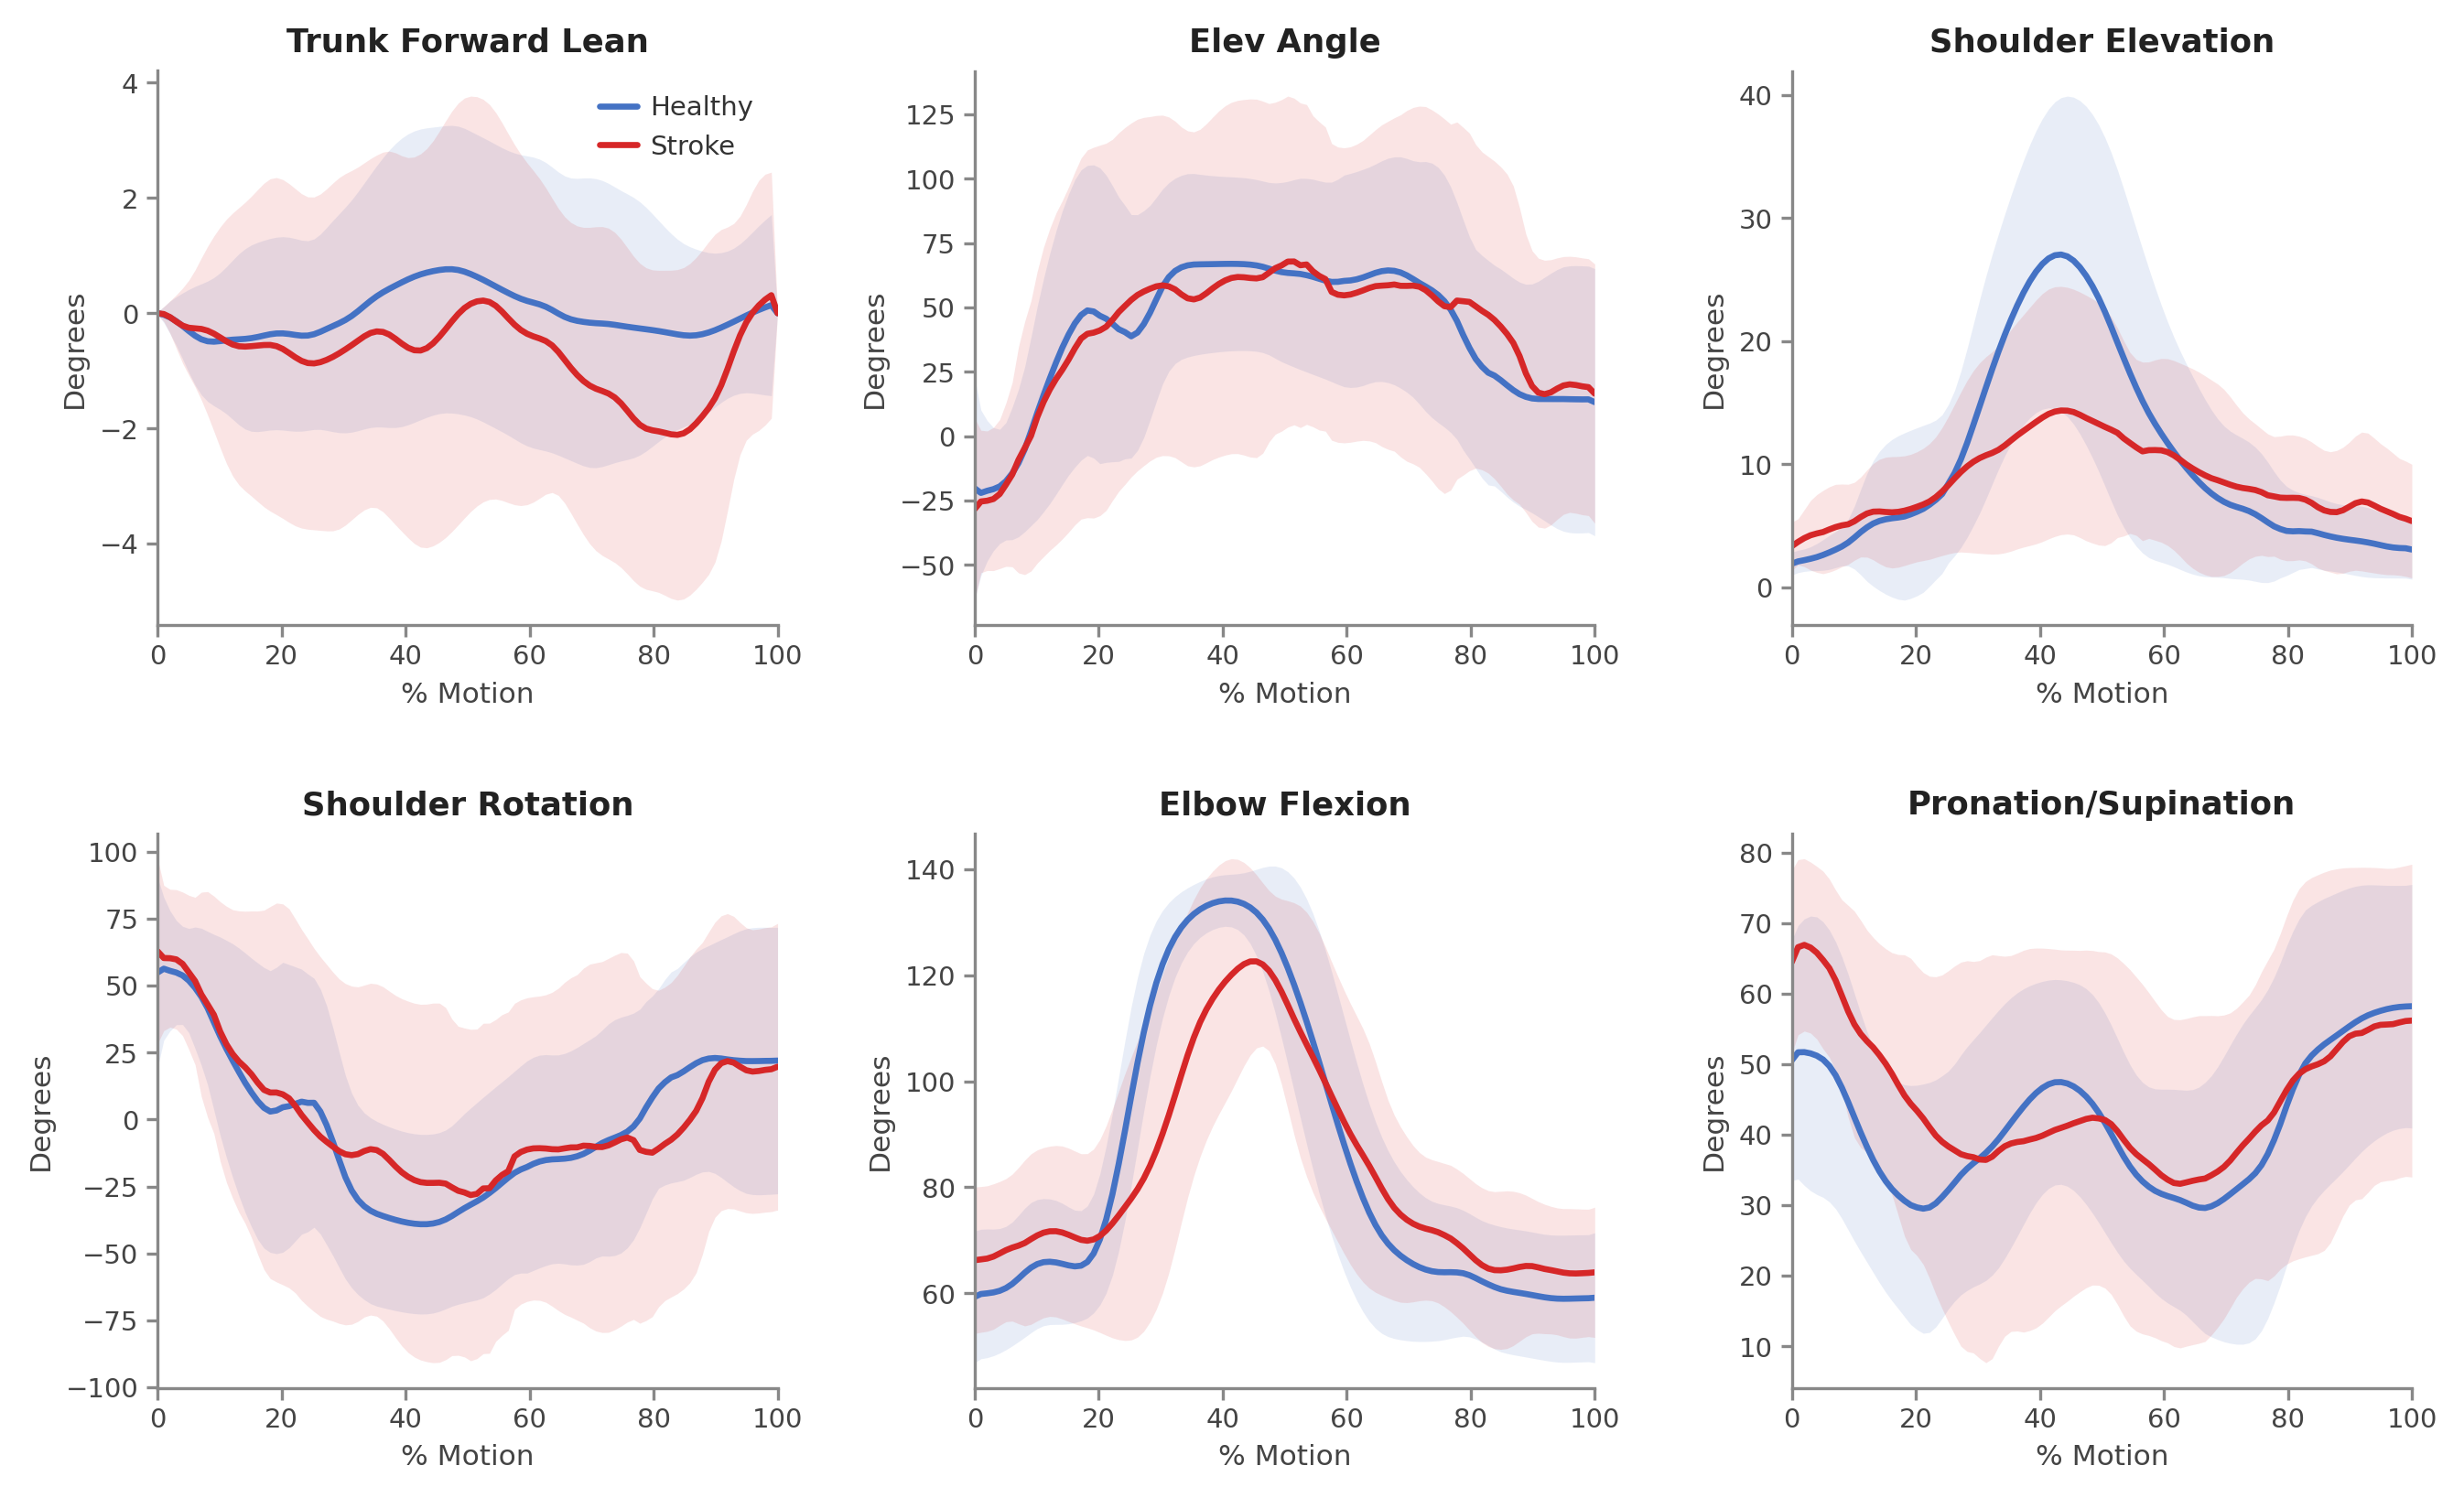
\includegraphics[width=\textwidth]{../figures_and_tables/joint_trajectories_weighted.png}
\end{center}

\clearpage
\begin{center}
    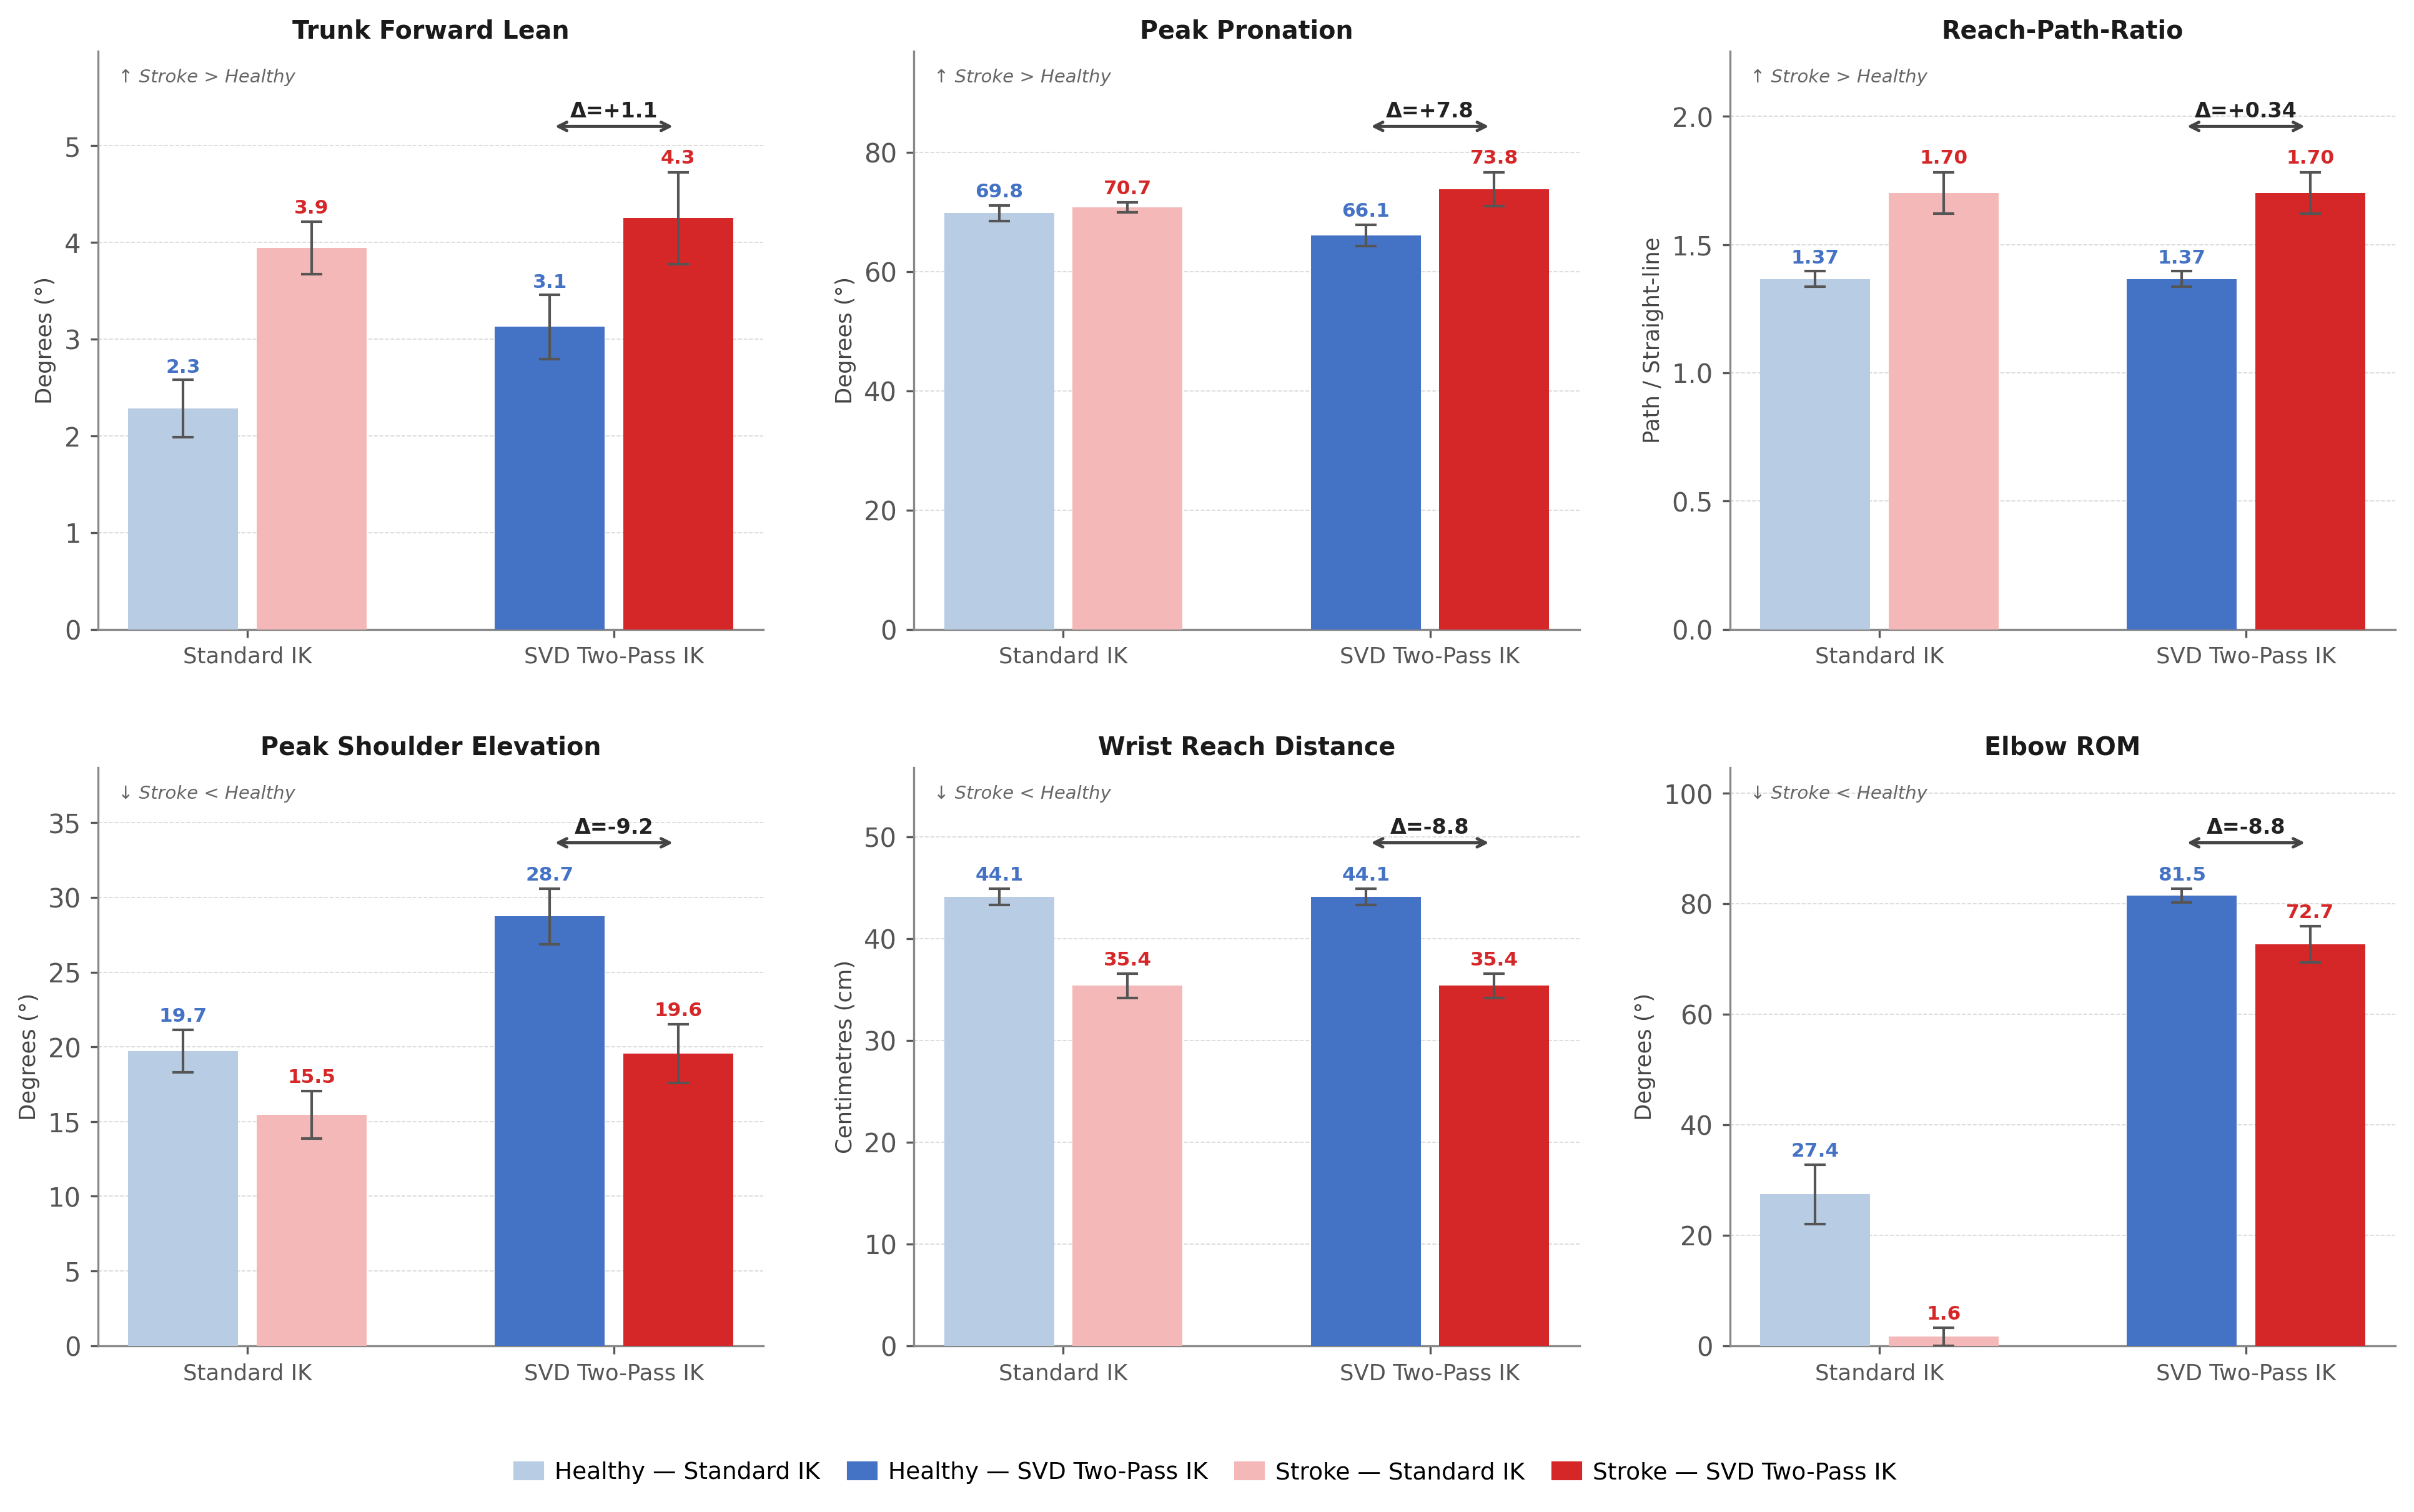
\includegraphics[width=0.8\textwidth]{../figures_and_tables/clinical_validation_results.png}
\end{center}

\clearpage
\begin{center}
    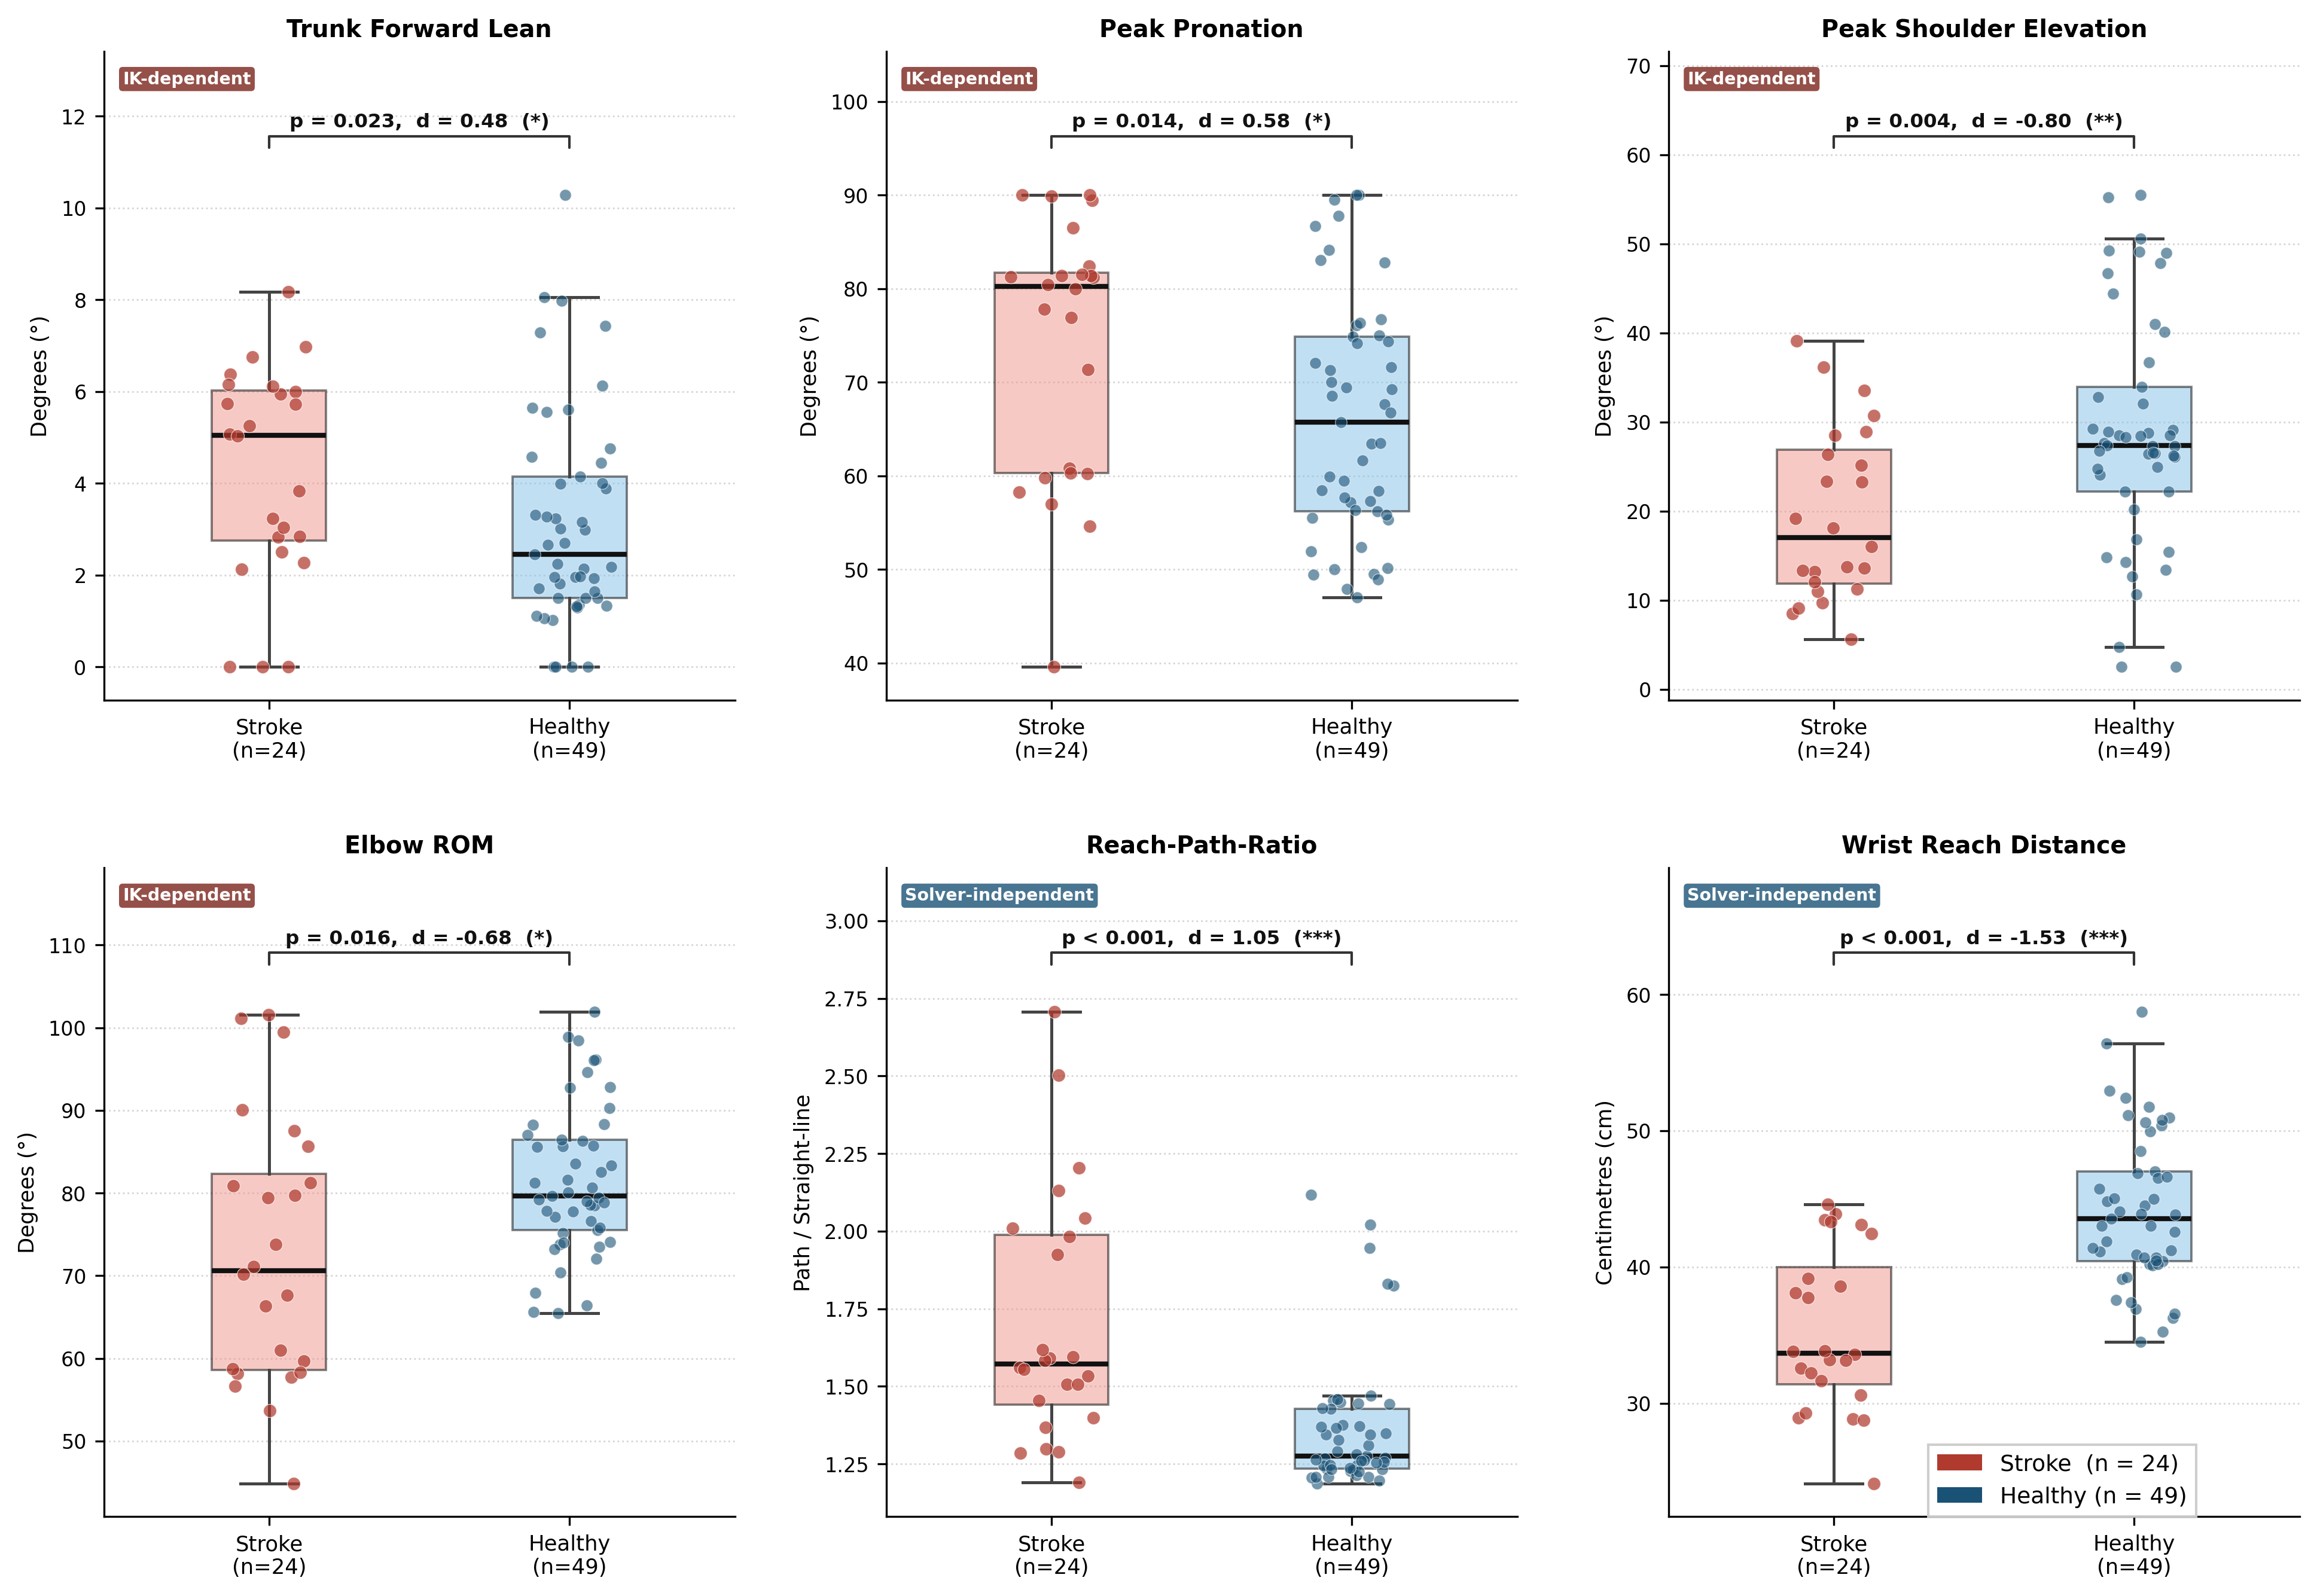
\includegraphics[width=\textwidth]{../figures_and_tables/final_5_metric_distribution.png}
\end{center}

\end{document}